\paragraph{QuizziPedia::Front-End::Controllers::ClickableAreaQuestionsController}
\begin{figure} [ht]
	\centering
	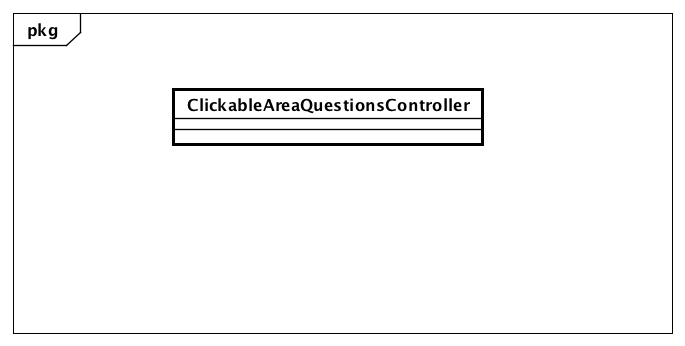
\includegraphics[scale=0.45]{UML/Classi/Front-End/QuizziPedia_Front-end_Controller_ClickableAreaQuestionsController.png}
	\caption{QuizziPedia::Front-End::Controllers::ClickableAreaQuestionsController}
\end{figure} \FloatBarrier
\begin{itemize}
	\item \textbf{Descrizione}: questa classe permette di gestire la creazione e la modifica di una domanda ad area cliccabile;
	\item \textbf{Utilizzo}: fornisce le funzionalità per inserire una nuova domanda ad area cliccabile nel database e per modificarne una esistente;
	\begin{itemize}
		\item \textit{IN} \texttt{ClickableAreaQuestionsModelView}: classe di tipo modelview la cui istanzazione è contenuta all'interno della variabile di ambiente \$scope di \textit{Angular.js\ped{G}}. All'interno di essa sono presenti le variabili e i metodi necessari per il \textit{Two-Way Data-Binding\ped{G}} tra la view \texttt{ClickableAreaQuestionsView} e il controller \texttt{ClickableAreaQuestionsController};
		\item \textit{IN} \texttt{QuestionService}: questa classe permette di:
		\begin{itemize}
			\item Ottenere una domanda attraverso il metodo dedicato;
			\item Caricare una domanda modificata;
			\item Caricare una nuova domanda.
		\end{itemize}
		\item \textit{IN} \texttt{QuestionItemModel}: questa classe rappresenta il modello di una domanda;
	\end{itemize}
	\item \textbf{Attributi}:
	\begin{itemize}
		\item \texttt{-} \texttt{\$scope: \$scope} \\
		Campo dati contenente un riferimento all’oggetto \$scope creato da \textit{Angular\ped{G}}, viene utilizzato come mezzo di comunicazione tra il controller e la view. Contiene gli oggetti che definiscono il model dell’applicazione;
		\item \texttt{-} \texttt{QuestionItemModel: QuestionItemModel} \\
		Campo dati che si riferisce alla classe che rappresenta il modello della classe;
		\item \texttt{-} \texttt{\$mdDialog: \$mdDialog} \\
		Campo dati contenente un riferimento al servizio della libreria \textit{Material for Angular\ped{G}} che permette di creare delle componenti a popup;
		\item \texttt{-} \texttt{QuestionService: QuestionService}: \\
		Campo dati contenente un riferimento al servizio che si occupa della gestione delle informazioni legate alle domande;
		\item \texttt{-} \texttt{Upload: Upload} \\
		Campo dati contenente un riferimento alla libreria \textit{ng-file-upload\ped{G}} necessaria per il caricamento della foto profilo dell'utente;
		\item \texttt{-} \texttt{\$timeout: \$timeout} \\
		Campo dati contenente il riferimento all'oggetto globale \$timeout creato da \textit{Angular.js\ped{G}}. 
		Il valore di ritorno di una chiamata alla funzione di \texttt{\$timeout} è una promise, la quale sarà risolta quando avverrà il ritardo e la funzione di timeout eseguita; 
		\item \texttt{\$routeParams: \$routeParams} \\
		Campo dati contenente il riferimento all'oggetto globale \$routeParams creato da \textit{Angular.js\ped{G}}. Tale servizio permette di recuperare il set di variabili presenti nell'url; 
	\end{itemize}
	\item \textbf{Metodi}:
	\begin{itemize}
		\item \texttt{+} \texttt{ClickableAreaQuestionsController(\$scope: \$scope, QuestionItemModel: QuestionItemModel, \$mdDialog: \$mdDialog, QuestionService: QuestionService, Upload: Upload, \$timeout: \$timeout, \$routeParams: \$routeParams)} \\ 
		Metodo costruttore della classe. Se in \texttt{\$routeParams} sarà presente il codice univoco che rappresenta una domanda e di questa il creatore è l'utente autenticato, allora verrà scaricato attraverso il \texttt{QuestionService} il contenuto della domanda così da poterlo modificare. In caso contrario verrà mostrato un errore attraverso \texttt{\$mdDialog} indicando che i privilegi per tale operazione sono negati. Nel caso in cui non ci sarà tale parametro in \texttt{\$routeParams} verrà caricata la view vuota così da poter creare una nuova domanda; \\
		\textbf{Parametri}:
		\begin{itemize}
			\item \texttt{\$scope: \$scope} \\
			Parametro contenente un riferimento all’oggetto \$scope creato da \textit{Angular\ped{G}}, viene utilizzato come mezzo di comunicazione tra il controller e la view. Contiene gli oggetti che definiscono il model dell’applicazione;
			\item \texttt{QuestionItemModel: QuestionItemModel} \\ 
			Parametro che si riferisce alla classe che rappresenta il modello della classe;
			\item \texttt{\$mdDialog: \$mdDialog} \\
			Parametro contenente un riferimento al servizio della libreria \textit{Material for Angular\ped{G}} che permette di creare delle componenti a popup;
			\item \texttt{QuestionService: QuestionService}: \\
			Parametro contenente un riferimento al servizio che si occupa della gestione delle informazioni legate alle domande;
			\item \texttt{Upload: Upload} \\
			Parametro contenente un riferimento alla libreria \textit{ng-file-upload\ped{G}} necessaria per il caricamento della foto profilo dell'utente;
			\item \texttt{\$timeout: \$timeout} \\
			Parametro contenente il riferimento all'oggetto globale \$timeout creato da \textit{Angular.js\ped{G}}. 
			Il valore di ritorno di una chiamata alla funzione di \texttt{\$timeout} è una promise, la quale sarà risolta quando avverrà il ritardo e la funzione di timeout eseguita; 
			\item \texttt{\$routeParams: \$routeParams} \\
			Parametro contenente il riferimento all'oggetto globale \$routeParams creato da \textit{Angular.js\ped{G}}. Tale servizio permette di recuperare il set di variabili presenti nell'url; 
		\end{itemize}
		\item \texttt{+} \texttt{submitQuestion(): void}\\ 
		Metodo che gestisce l’evento click sul pulsante di conferma sulla domanda. Raccoglie i dati dal modelview e li manda al server attraverso \texttt{QuestionService}. Poi verrà effettuato il redirect alla pagina di gestione delle domande oppure al questionario che si stava creando; 
		\item \texttt{+} \texttt{choseThatPoint(x:Integer, y: Integer): void}\\
		Metodo che gestisce l’evento click su un punto dell'immagine. Una volta selezionato esso verrà inserito nell'array di punti; \\
		\textbf{Parametri}:
		\begin{itemize}
			\item \texttt{x: Integer} \\
			Parametro contenente la coordinata x del punto;
			\item \texttt{y: Integer} \\ 
			Parametro contenente la coordinata y del punto;
		\end{itemize}
	\end{itemize}
\end{itemize}

